\section{Veto Detector}
\label{sec:Veto}

%---
\subsection{Overall Design}

Benefiting from the implementation of a \pDUNE-like \AAr\ cryostat, the Veto detector will utilize \AAr\ as the scintillation material. The Veto detector is composed of three separate volumes; a passive octagonal acrylic shell loaded with gadolinium called the GdA and mounted around the \TPC\ and providing $4-~\pi$ coverage, a  \DSkVetoIABThickness\ thick inner volume of active liquid \AAr\ called the Inner Argon Buffer (IAB) and sandwiched between the \TPC\ vessel and the GdA, a  \DSkVetoOABThickness\ thick outer active volume of \AAr\ called the Outer Argon Buffer (OAB) contained between the GdA and the outer copper Faraday Cage.  The Faraday Cage will contain the Veto and \TPC\ and optically and electrically isolate them from the remaining outermost \AAr\ volume contained within the cryostat.  A schematic drawing of the Veto concept is shown in the left side of Figure~\ref{fig:VetoScheme}, as well as a 3D cut-away drawing which presents the preliminary design.

\begin{figure}[!t]
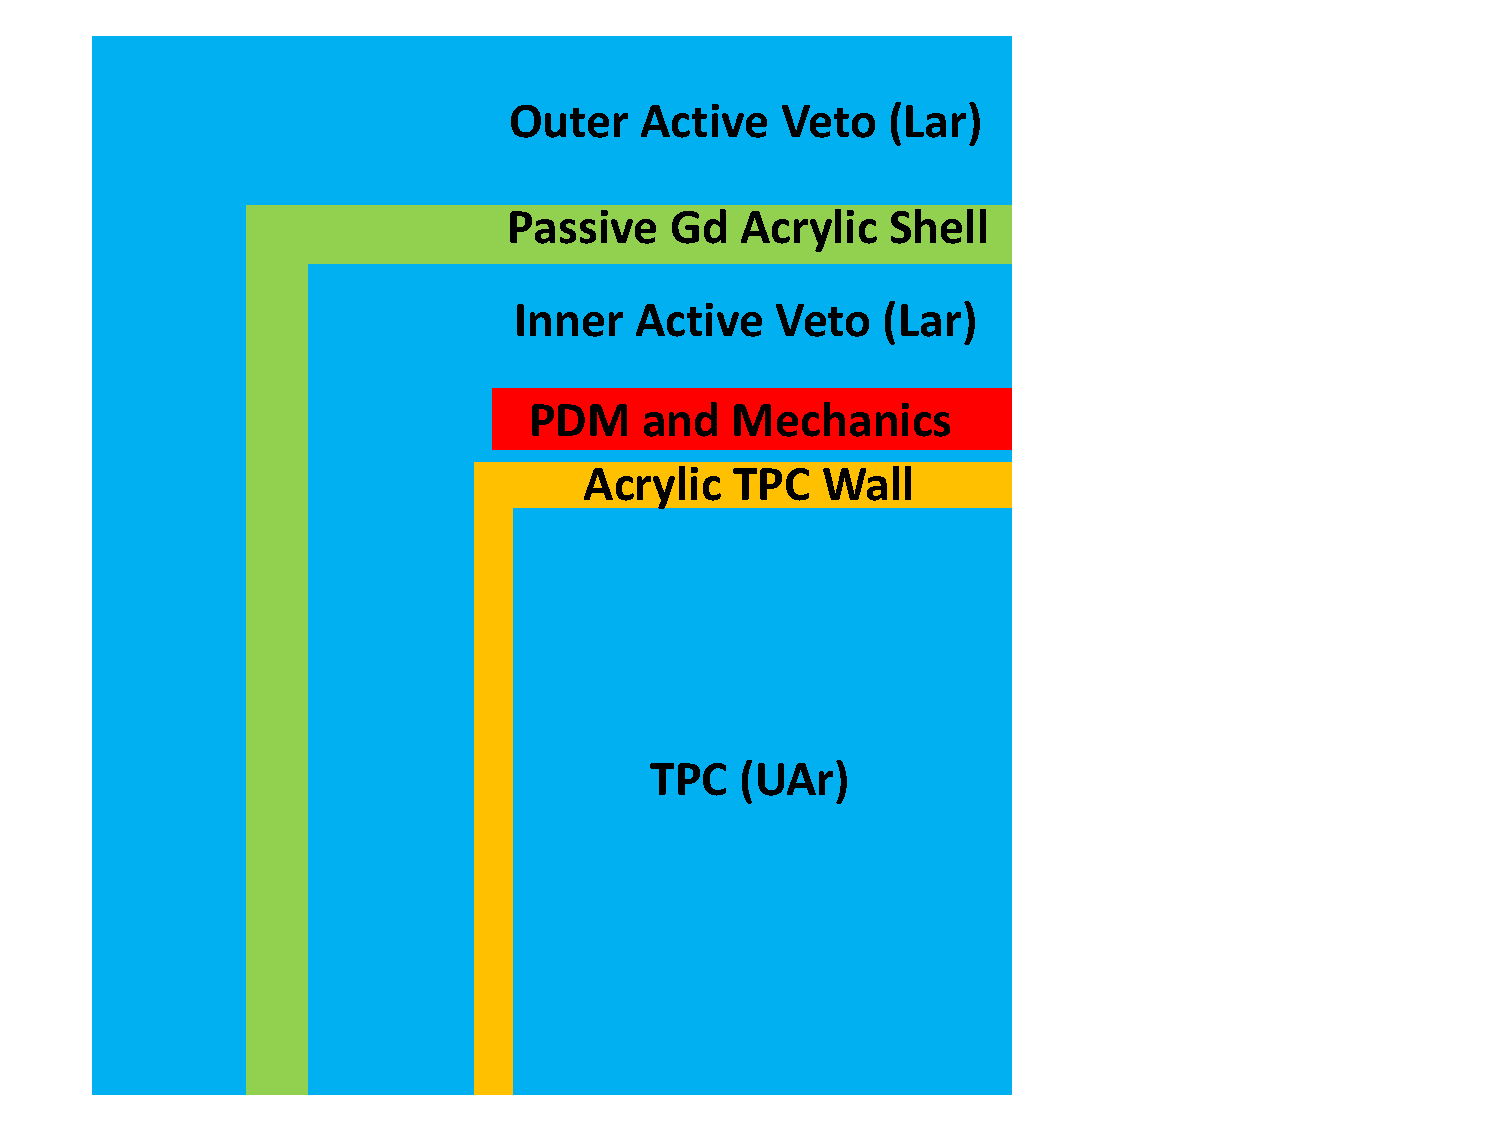
\includegraphics[height=0.43\textheight]{./Figures/Veto.pdf}
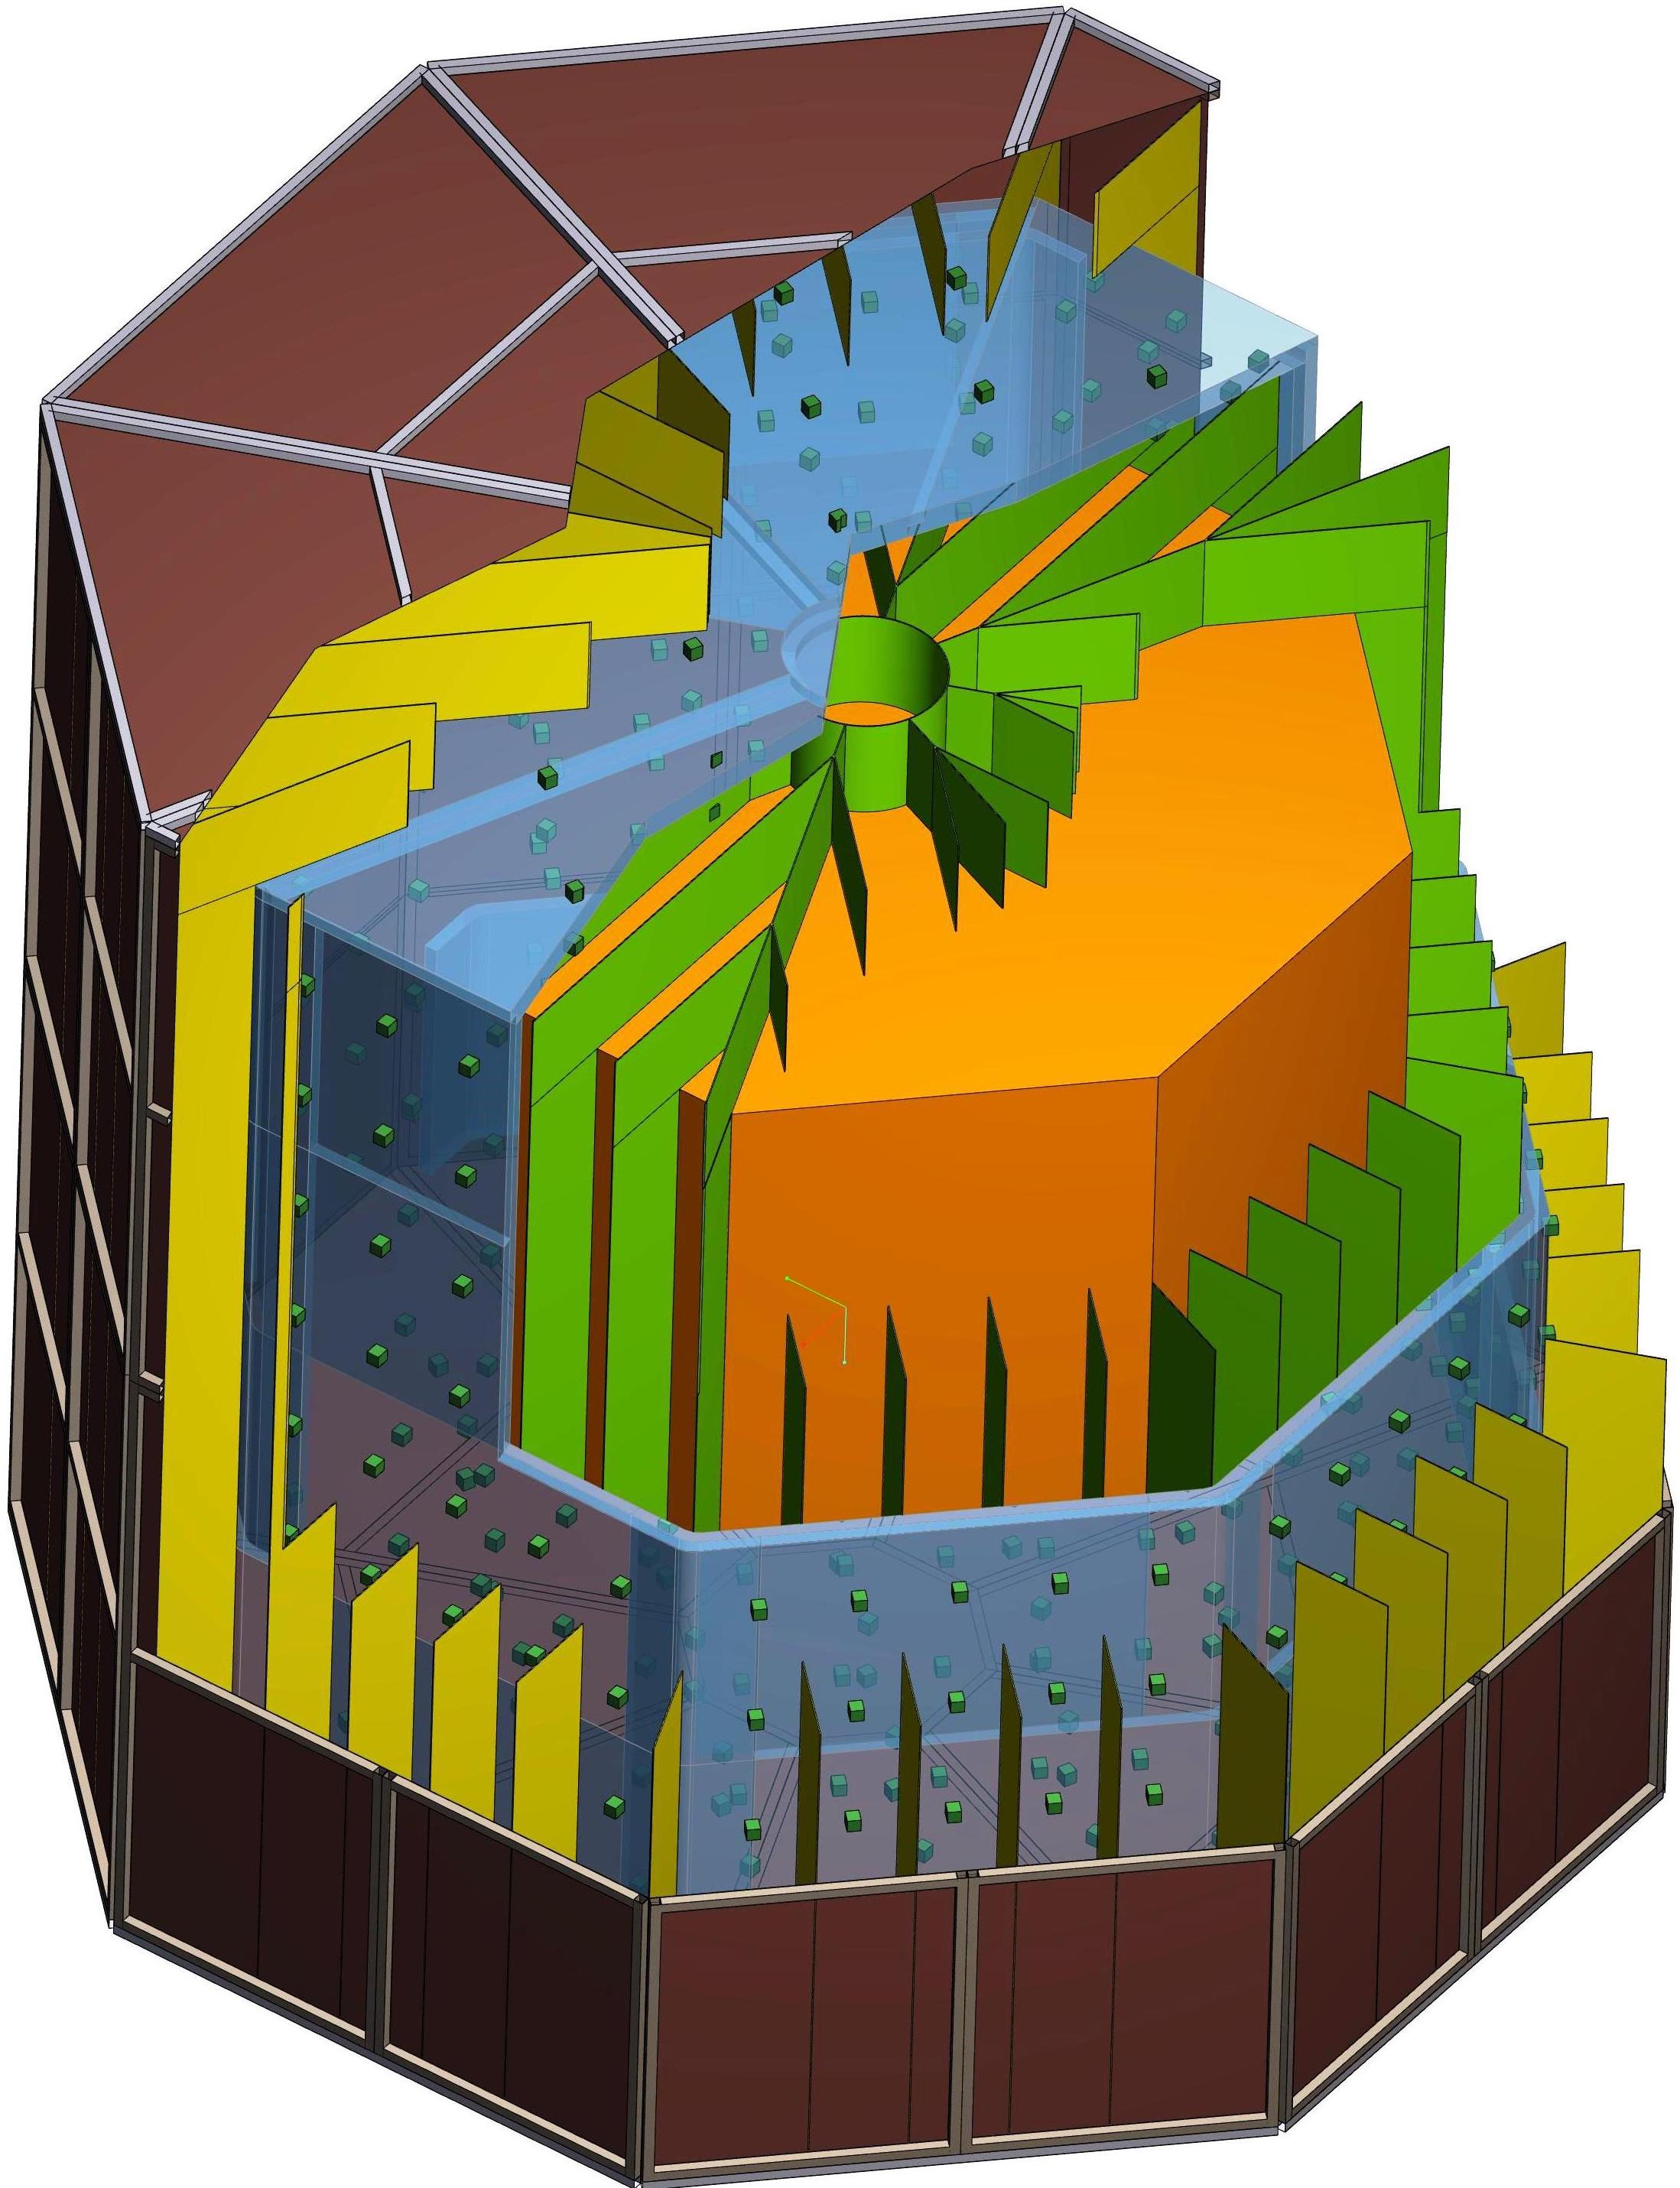
\includegraphics[height=0.43\textheight]{./Figures/Veto-CutAway.jpg}
\caption[Schematic and 3D cut-away view of the \DSks\ veto detector]{{\bf Left:} schematic conceptual view of the veto detector.  {\bf Right:} 3D cut-away view of the \DSks\ veto detector.}
\label{fig:VetoScheme}
\end{figure}

The required thickness of both the \IAB\ and \OAB\ of about \DSkVetoOABThickness\ has been determined by MC simulation. The required thickness of the \GdAS\, determined by the same simulation,  is about \DSkVetoGdASThickness\ with a required \ce{Gd} loading of \DSkVetoGdPercentage\ by weight.  The \GdAS\ moderates neutrons emitted from all of the detector materials, particularly from the ones which make-up and surround the \LArTPC, while also enhancing the neutron capture probability with the inclusion of the \ce{Gd}.  The capture of the neutron on a \ce{Gd} nucleus results in the emission of multiple \grs.  These \grs\ interact in the \IAB\ and \OAB, their detection efficiency setting the required \GdAS\ thickness and \ce{Gd} loading fraction, as well as the minimum required \IAB\ and \OAB\ thickness.  \grs\ are detected by use of scintillation light emitted by the liquefied \AAr\ in both the \IAB\ and \OAB. 

The Veto will be built coupling \GdAS\ plates each one with thickness of \DSkVetoGdAsSheetThickness\, that is half of the nominal one of \DSkVetoGdASThickness\, with liquid Argon flowing in between. The reference size of each vertical plate is approximately 60 X 200 cm. Plates of proper size and shape will be mounted on top and bottom covering the TPC in all the directions.
Proper holes for cables and services will be allocated.

Vertical segmentation of the \IAB\ and \OAB\ is foreseen to reduce the pile-up rate of \ce{^39Ar} events from the \AAr.  The concept of this is shown in the cut-away view of the detector in the right panel of Figure~\ref{fig:VetoScheme}, while the exact details are still being optimized by use of the Monte Carlo simulation. 

\SiPMs\ will be mounted on the sides of the \GdAS\ such that they are facing both the \IAB\ and \OAB: we foresee about \DSkVetoTotalPDMs\ \SiPMs\ in total, \DSkVetoIABPDMs\ of them facing the \IAB\ and \DSkVetoOABPDMs\ the \OAB\. The basic detector element is the same \DSkPdm\ used in the \TPC, but with a different front-end board coupled to it that is optimized for the geometry of the Veto detector. 
The baseline option is the use of a front end board realized with a custom ASIC (integrated electronics) developed
within the DarkSide collaboration.
 Very promising results in terms of signal to noise have been already obtained with 
a front end board equipped with a prototype ASIC coupled to a tile at cryogenic temperature (see Fig.~\ref{fig:asic_finger}.

\begin{figure}[!t]
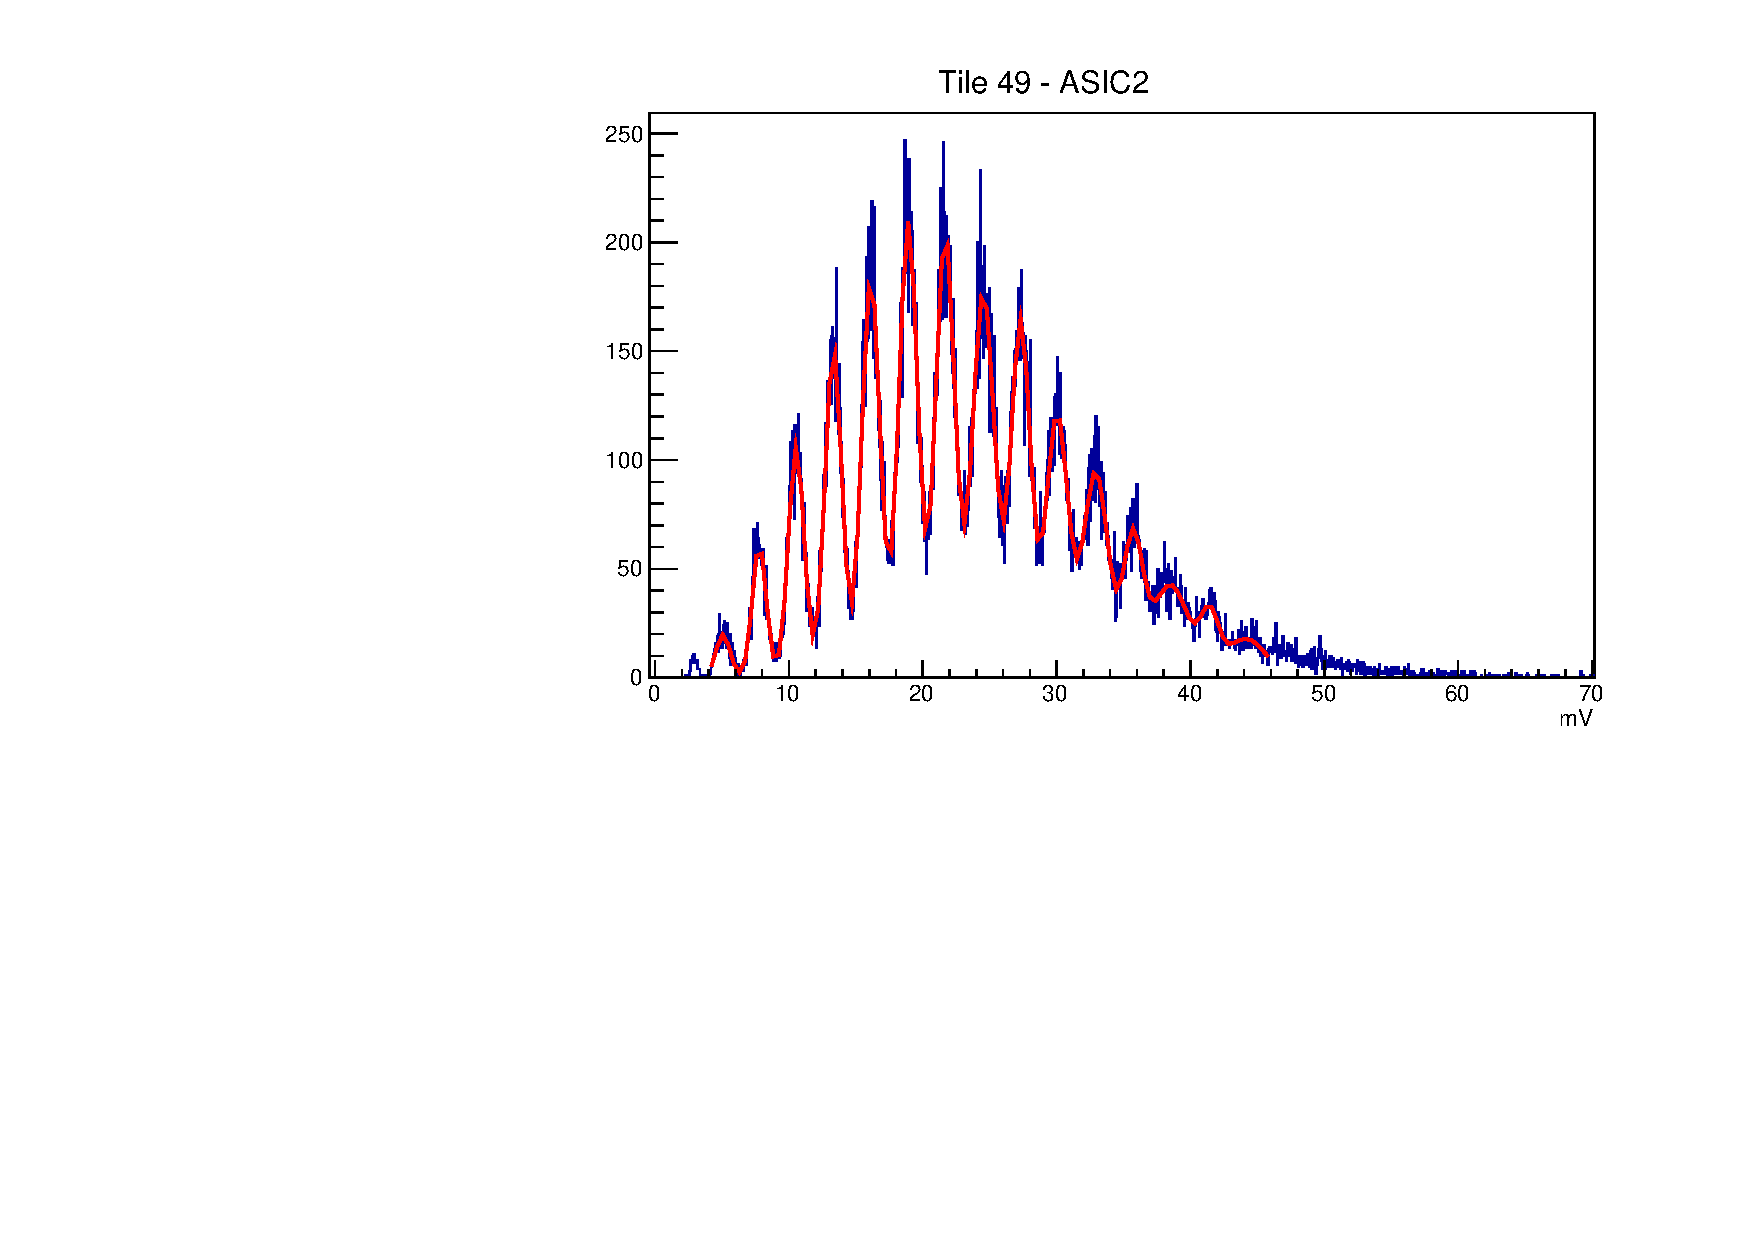
\includegraphics[height=0.3\textheight]{./Figures/Laser7_8_15peaks.pdf}
\caption[Preliminary Veto ASIC front-end performance.]{Results of tests of the Veto ASIC prototype front-end with tile 49 (single doping) in liquid argon with illumination from laser pulses.
Peaks corresponding to up 15 photo-electrons are clearly resolved. In these test conditions we had 2.8 mV/phe.}
\label{fig:asic_finger}
\end{figure}

Further tests are in progress whose results, together with Montecarlo simulation of the VETO optical response, will set the final specifications (mostly about the necessary dynamic range) of the next ASIC prototype that will be produced and tested in the following months.
About 10-20 \SiPMs\ will be mounted of each plate and there will be a dedicated control board (called Veto Steering Module) for each plate carrying the bias to \SiPMs\ and control signals. Each plate together with its electronics is then  the basic modular unit of the Veto (Veto Detector Unit- VDU).

All of the inner surfaces of the Veto, including the external walls of the \TPC\ and the walls of the vertical sectors, will be covered with reflector foils coated with wavelenght shifter (TPB), so that the VUV argon scintillation light is shifted to longer wavelengths where the \LAr\ is very transparent. This light is then trapped within a segment of the Veto detector by multiple reflections until it reaches a \SiPM. 
The use of reflector foils coated with TPB is a well proven technology. However, some challenges are related to the need to evaporate TPB on very large surfaces  (of the order of many hundreds square meters), therefore we are also investigating the possibility to use PEN (polyethylene naphthalate) in alternative to TPB.  PEN  reflector foils can be laminated, thus offering a simplified procedure during the preparation and assembly phases of the VETO elements. Tests are in progress to confirm that the fluorescence yield~\cite{Kuzniak:2018dcf} of PEN matches our needs.

The optimal number of segments is being studied with Monte Carlo simulation. We expect no more than \DSkVetoMaxSectorPerSide\ segments for each edge of the octagon. The segments are not liquid tight to allow flow of the argon through them, with a dedicated fluid-dynamics simulation planned to be performed to ensure that the \LAr\ can be properly re-circulated throughout the proposed geometry.

The overall Veto detector design and the Monte Carlo simulation results will be validated using smaller prototype setups.  Due to the nested nature of the detector system, strategic planning for the detector integration is also a big part of the development planning.

This conceptual design promises to achieve the most important criteria for the \DSks\ detector, which is the efficient detection of neutrons such that no instrumental background interferes with the potential nuclear recoil signal from a \WIMP\ scattering off of an argon nucleus.   The design concept is scalable and lends well to serve as the basis for the future \ArgoTotalMass\ scale detector designed to collect an exposure of \ArgoExposure\ in absence of instrumental background. The Veto design is based on elements which require no R\&D and therefore can be built out of materials already available, with the only exception being the gadolinium loaded acrylic. We have established good contacts and an agreement with a company available to test in its laboratory techniques to mix gadolinium compounds with liquid MMA before starting the polymerization process. Taking into account that we do not need  the final Gd-doped acrylic to be transparent to light (it acts only as passive neutron moderator), and that the homogeneity of the mixture is also not a critical parameter, several known difficulties related to metal loading into plastic scintillators are not an issue.
After the first laboratory tests, samples \DSkVetoGdAsSheetThickness\ thick, have been obtained realizing a dispersion of nano-grains of $Gd_2O_3$ in the MMA using the industrial production line.
Work is in progress to characterize the mechanical and cryogenic properties of the resulting material and also to select the producer of the Gadolinium compound with the radio-purity 
matching our needs.
%Monte Carlo simulation has also shown that an alternative solution can be implemented which uses gadolinium foils interleaved with thin acrylic layers.  it turns out that this does not spoil the performance of the Veto and is considered as a backup solution in case the R\&D for producing the mixture of Gd and MMA is not as successful as planned. We also note that the acrylic for the construction of the \LArTPC\ vessel and the \GdAS\ will be contributed by the IHEP group, which is preparing to start a much larger production for the JUNO experiment.  The acrylic radiopurity is reported to be close to that of Ref.~\cite{Nantais:2013jp}.  


%---
\subsection{Assembly}

The assembly sequence starts with the mounting of the bottom part of the GdAS along with its \DSkPdms. This component will rest on a stainless steel support structure (Veto support structure) that is itself supported by the cryostat floor via temporary feet. The \TPC\ is then lowered into its place above the bottom of the Veto detector. Once in place, the TPC is mechanically connected to the support structure of the Veto through mounting pillars. This choice has been driven by the aim of reducing the mass of the support structure of the TPC and avoiding relative movements between the TPC and the VETO during construction, commissioning and detector operation. 

Once the \TPC\ is fixed to the Veto support structure, the lateral panels of the GdAS and their \DSkPdms\ are mounted.  The vertical thin panels that divide the IAB into segments are then installed. The top GdAS panels are assembled next. Once the construction of the IAB is completed, \DSkPdms\ are installed on the external surfaces of the GdAS and the panels which divide the OAB into segments are integrated. Then the copper frames that are used as the main structure of the Faraday cage are installed in the outermost part of the Veto. Finally the Veto detector is hanged from the cryostat roof using a dedicated support structure and several Kevlar ropes. One the Veto detector construction is completed, the temporary pillars used to support the Veto on the cryostat floor during the construction are removed. 

\begin{figure}[!t]
%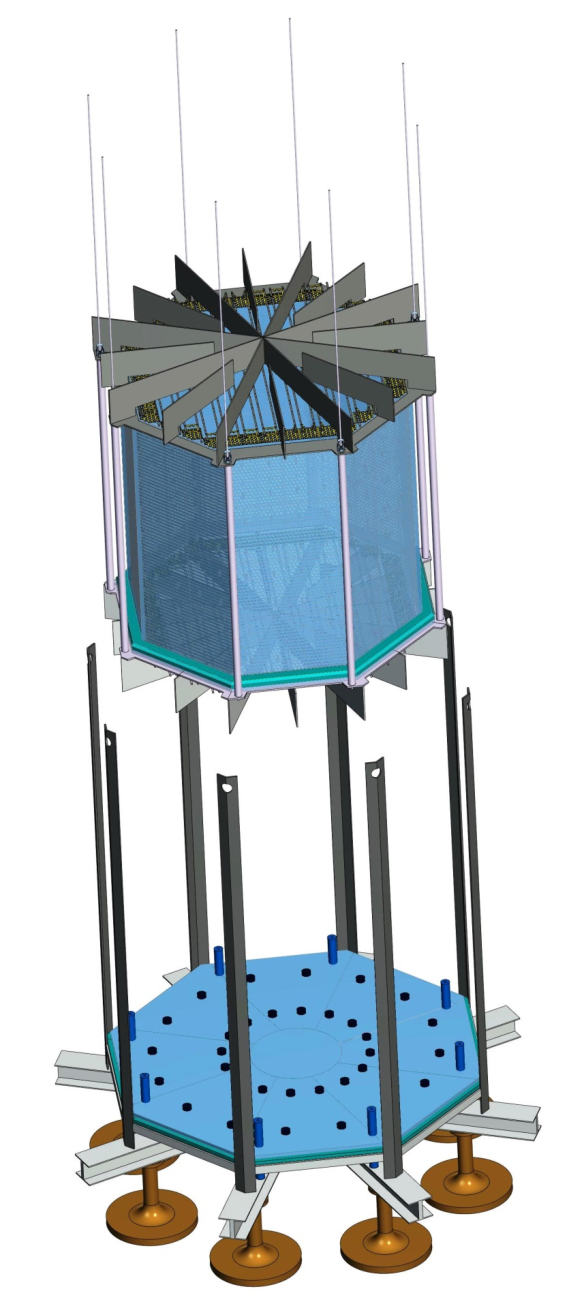
\includegraphics[height=0.75\textheight]{./Figures/Veto-Assembly.pdf}
%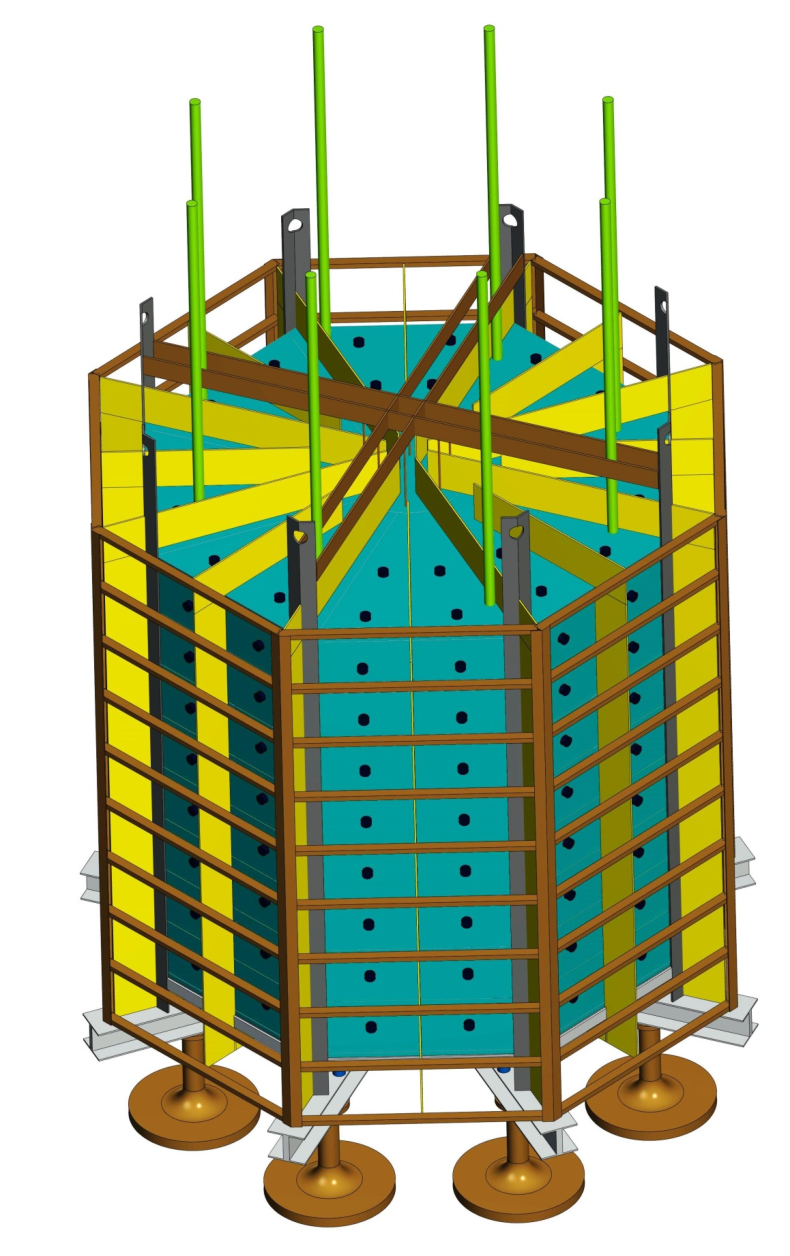
\includegraphics[height=0.75\textheight]{./Figures/Veto-Faraday.pdf}
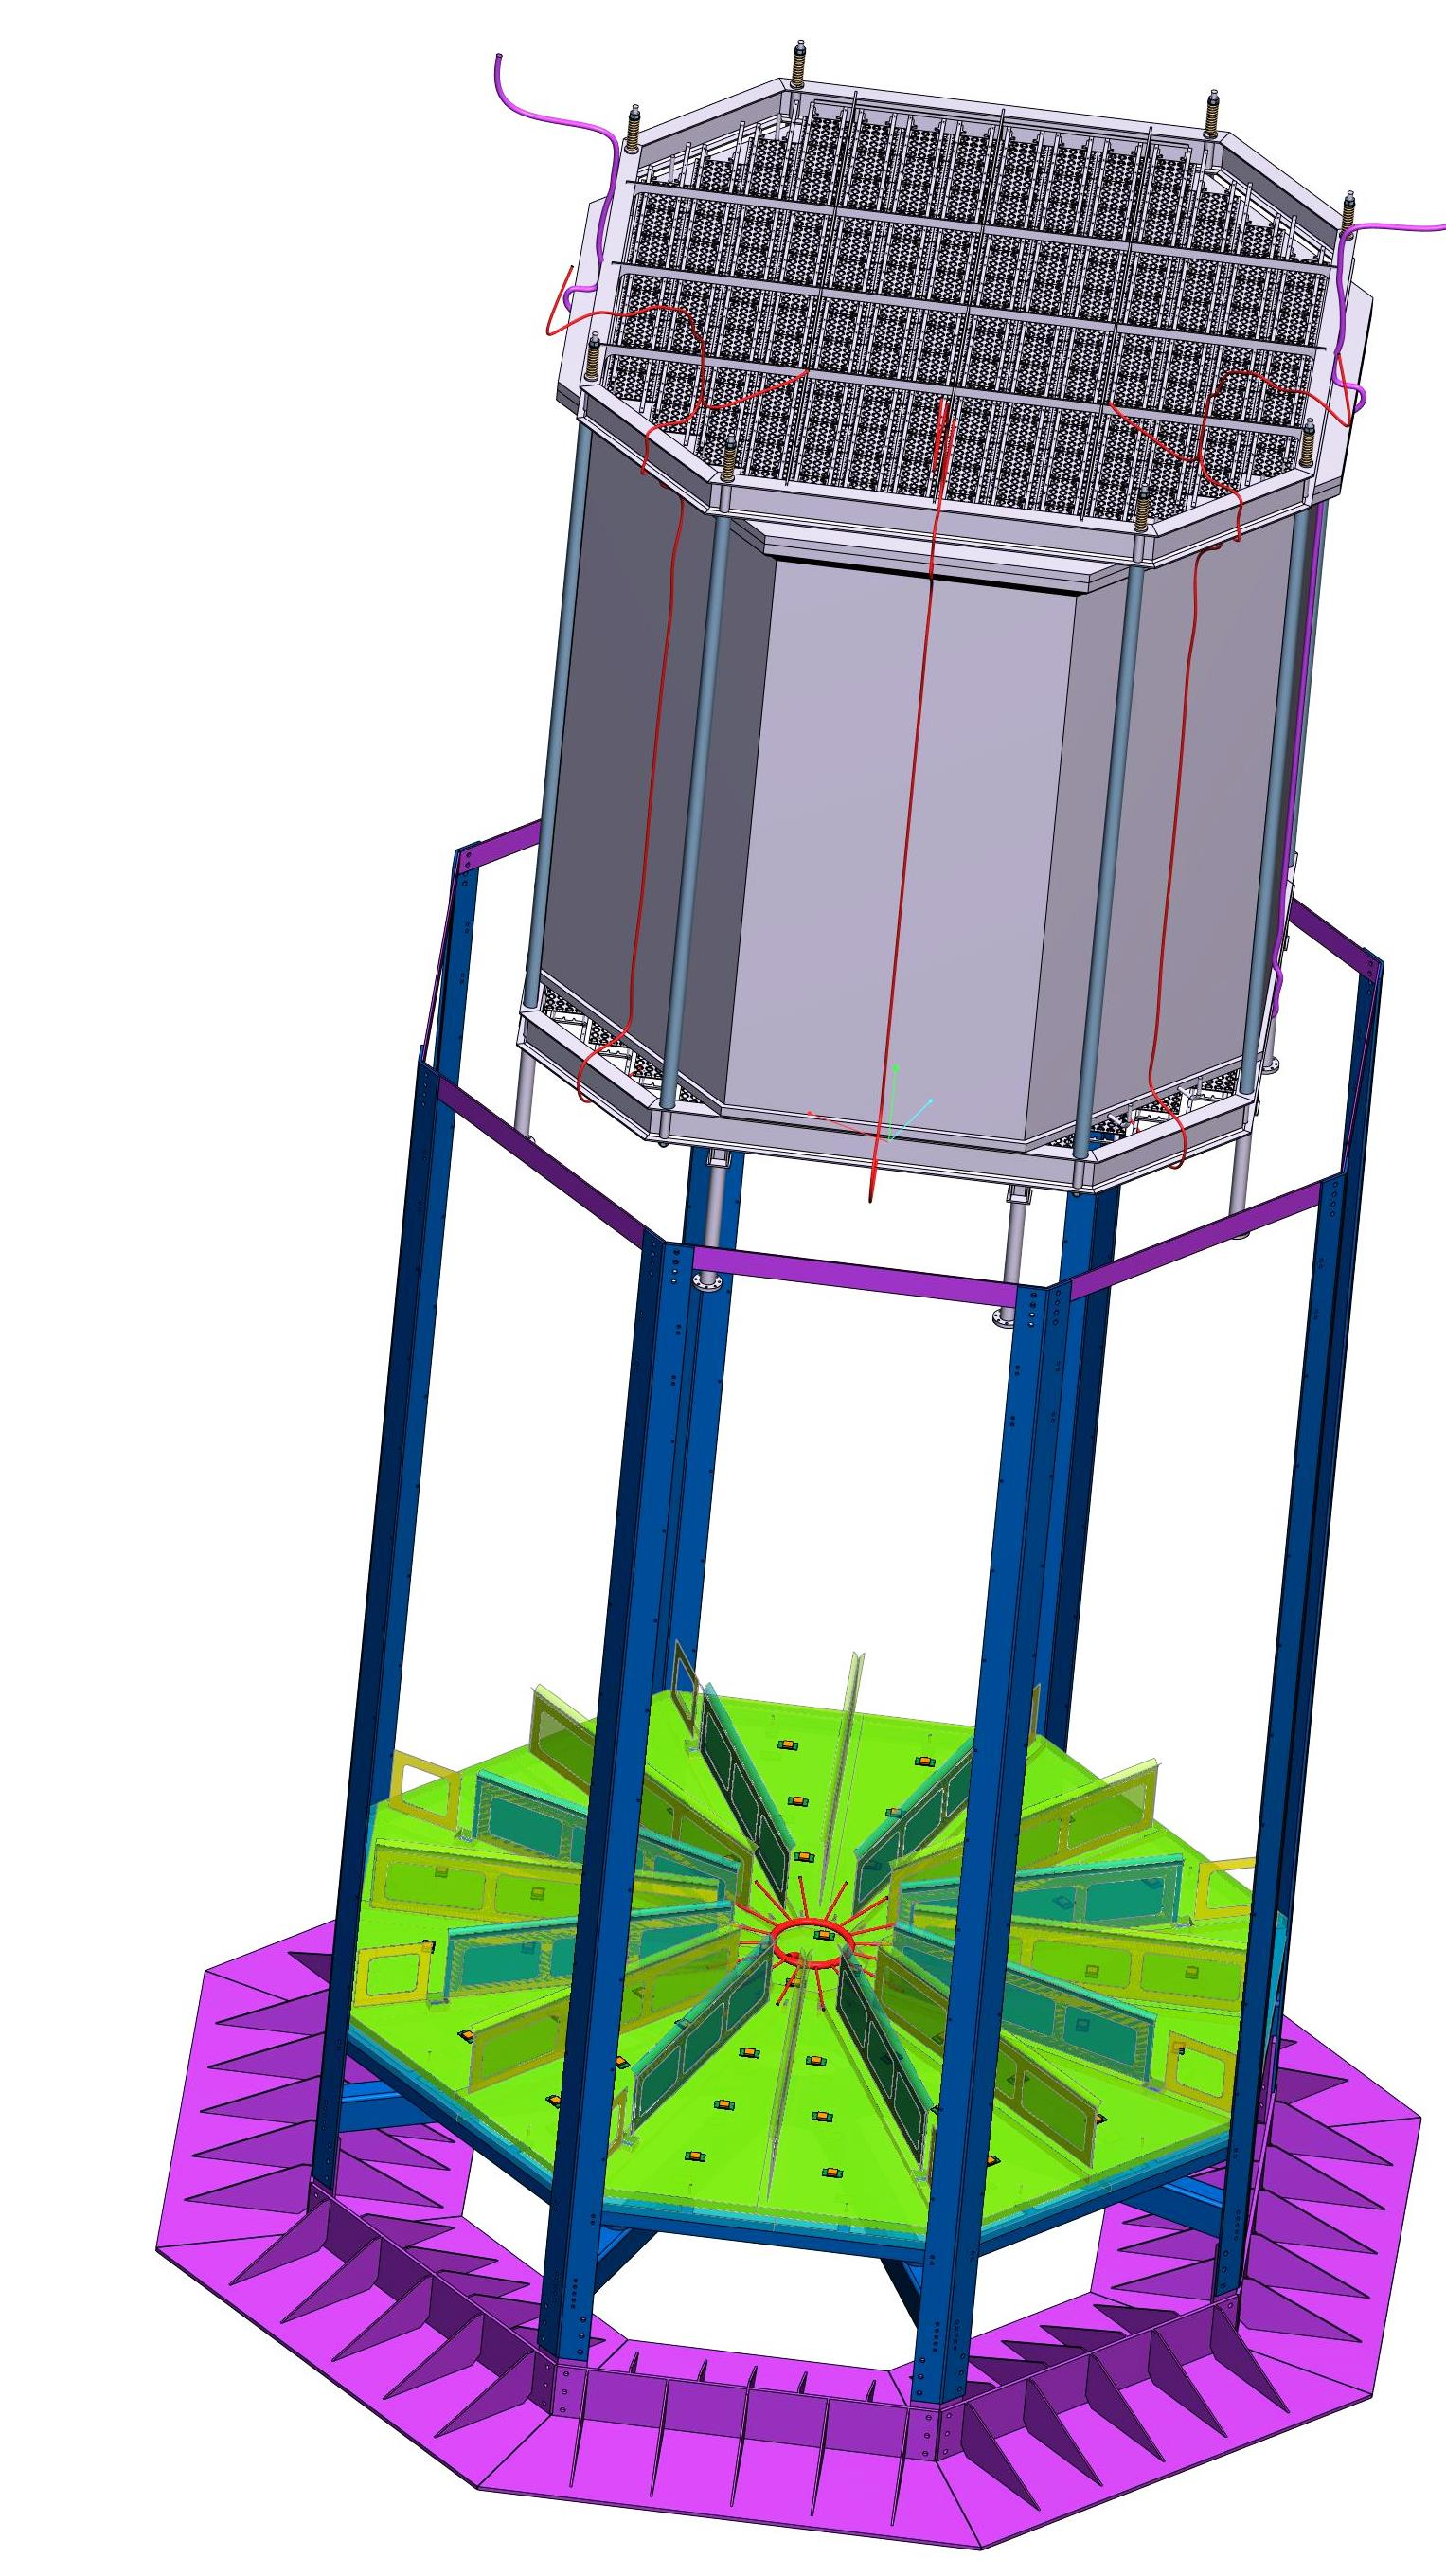
\includegraphics[height=0.4\textheight]{./Figures/Veto-Assembly_new.jpg}
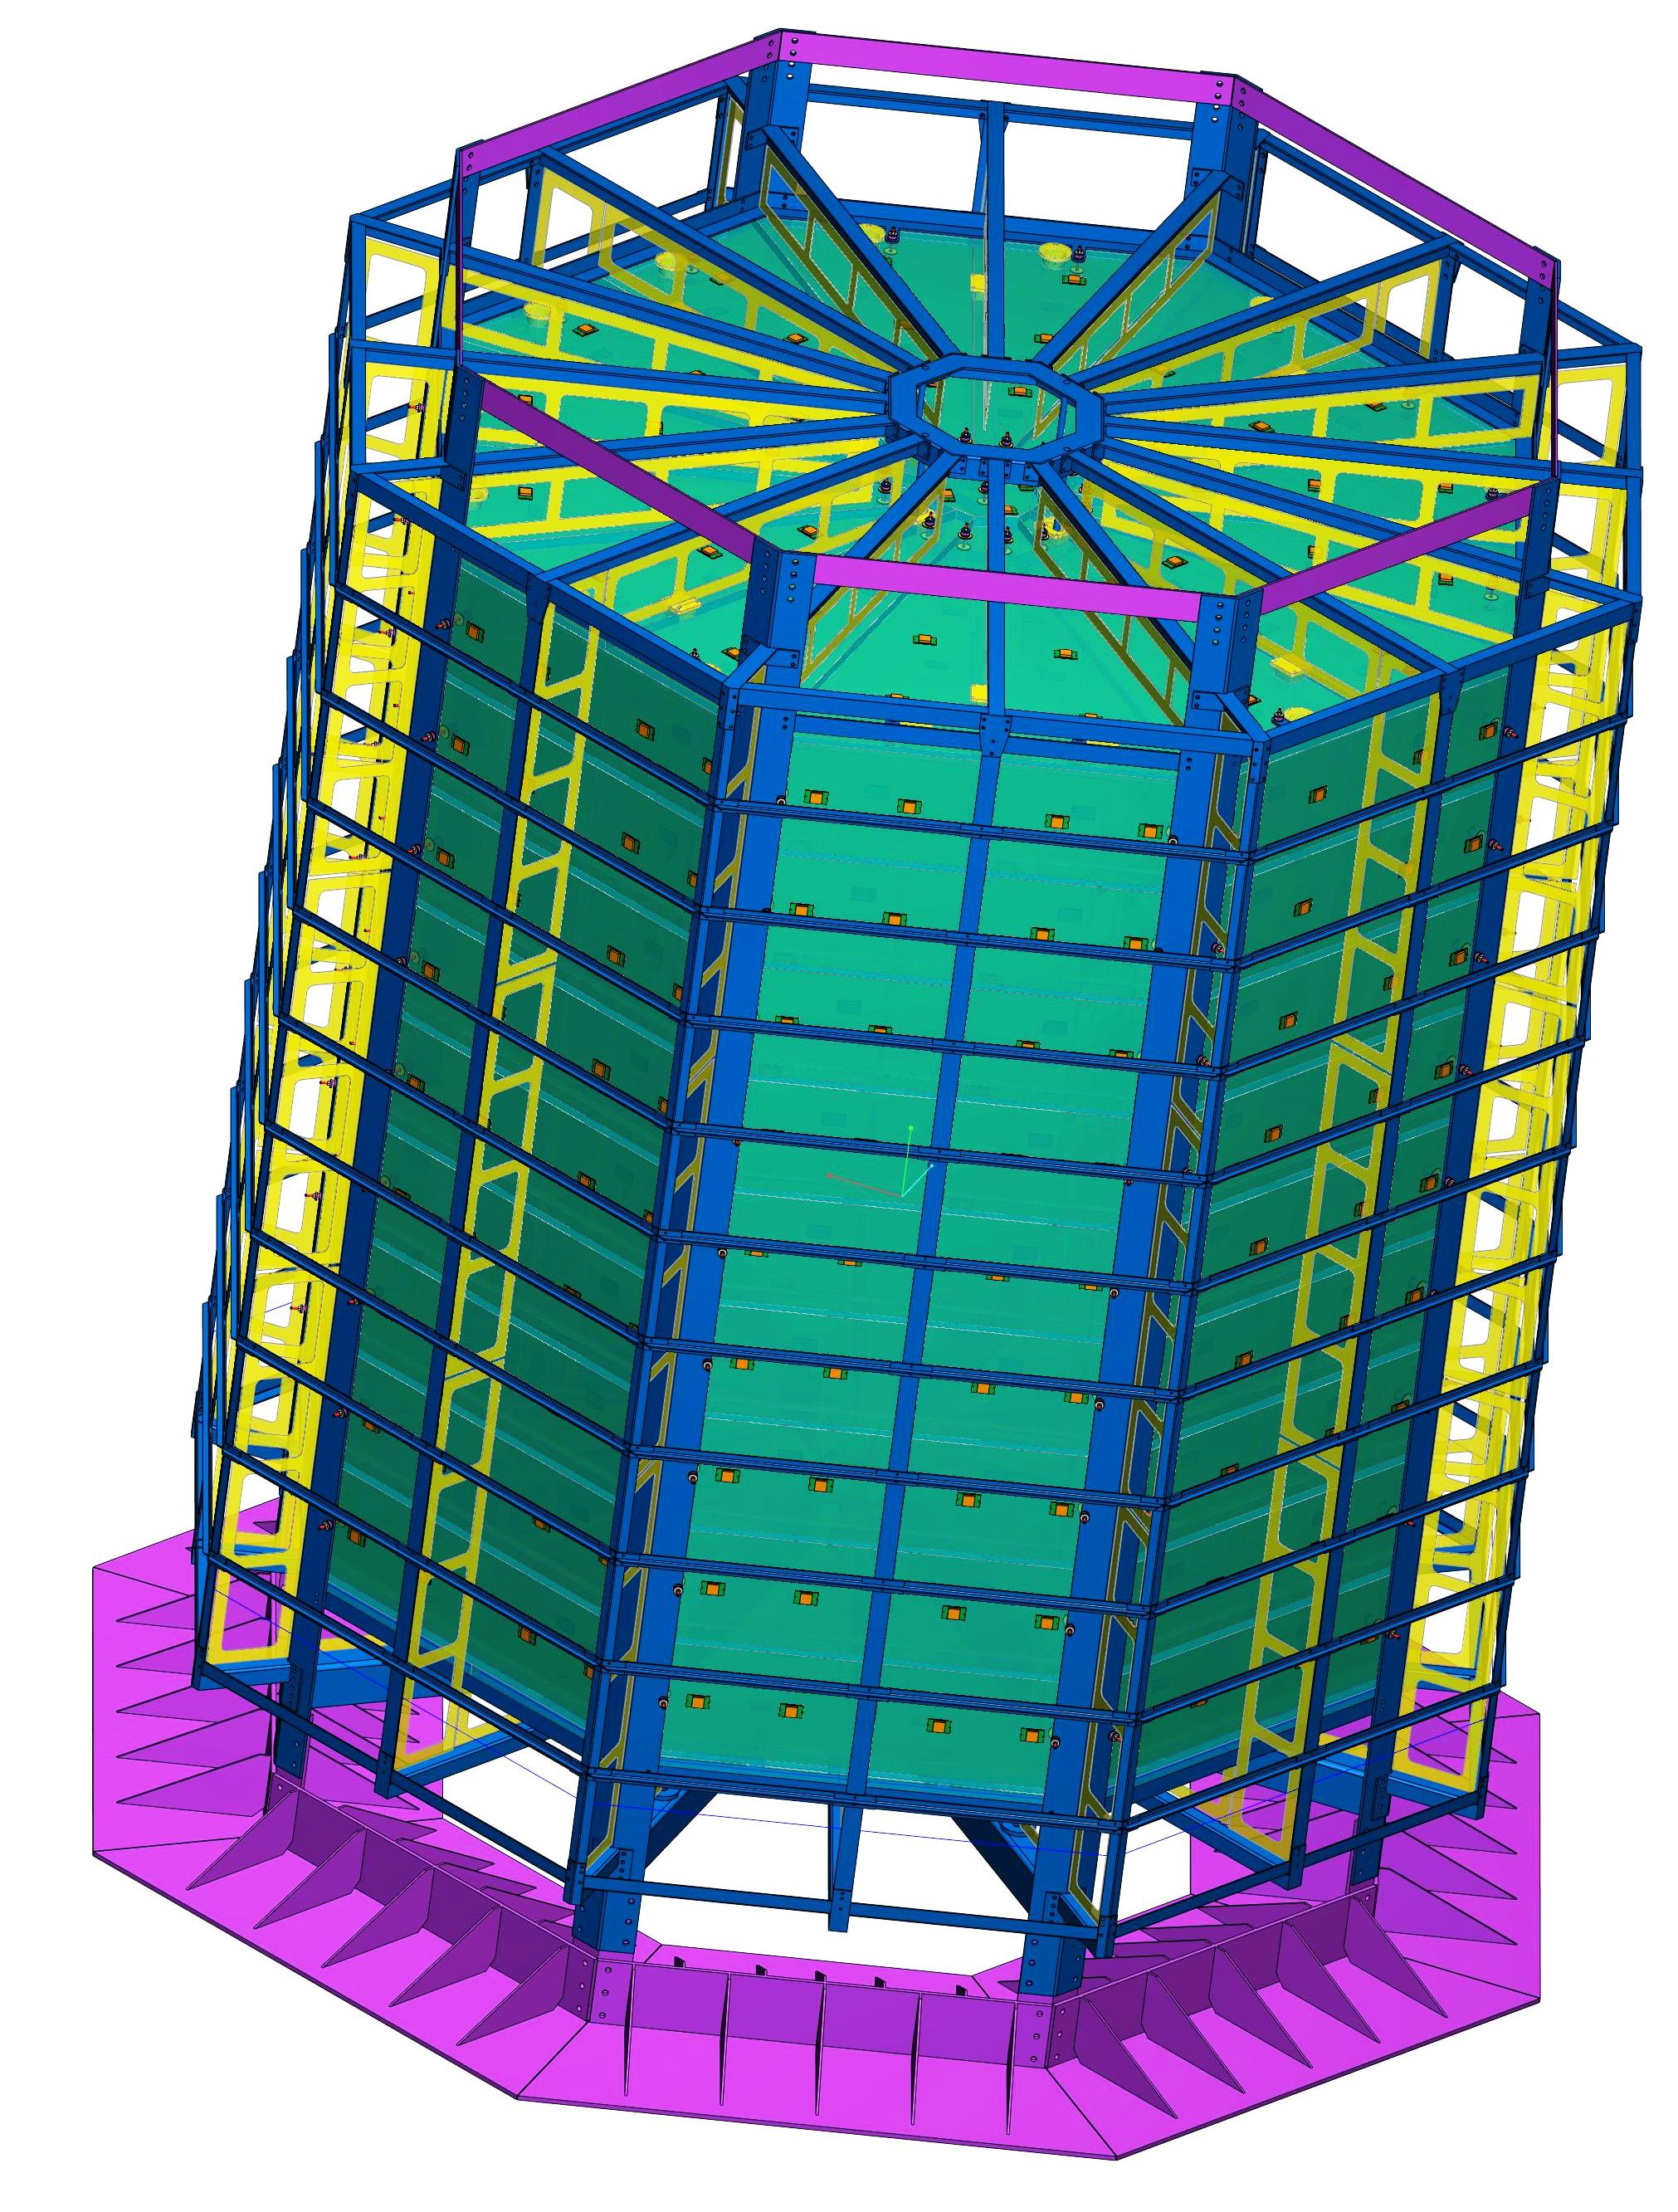
\includegraphics[height=0.4\textheight]{./Figures/Veto-Faraday_new.jpg}
\caption[3D drawings of the \DSks\ Veto detector.]{{\bf Right} Conceptual view of the placement of the \TPC\ within the Veto support structure. {\bf Left} 3D drawing of the \DSks\ Veto detector, along with the temporary bottom support structure used for assembly and the Faraday cage.}
\label{fig:VetoAssembly}
\end{figure}

%----
\subsection{Background Rejection}

The combination of the signals occurring inside the \IAB\ and \OAB, within a given time window, is used to tag and reject neutron captures.  If a neutron produces a signal in the \TPC, it will mimic that of a \WIMP\ signal, meaning that it produces a single energy deposit with energy in the range \DSkROIEnergyRange.  This also includes fiducial volume cuts which exclude events occurring at a distance from the \TPC\ walls less than \DSkVetoFVTPCcut\ in the radial direction and less than \DSkVetoFVTPCcutz\ from the top and bottom.  For events that pass this fiducialization, the Veto is then searched within a time window of  \DSkVetoTimeCut\ around the \TPC\ trigger time. To minimize dead time losses due to $\beta$-decay from \ce{^39Ar} in the veto filled with \AAr,  a \ABSingleThreshold\ threshold is set for each of the two parts of the Veto detector, while a lower \ABCoincidenceThreshold\ threshold is set for events with coincidence signals in both parts of the Veto detector.

The design of the Veto and the choice of all the materials used to build the entire detector are set by the requirement of having less than \BackgroundFreeRequirement\ untagged neutrons during the total exposure of \DSkExtendedExposure.  The radioactive contamination of the materials used to build the Veto is therefore also considered and limits are set by requiring that the corresponding neutron background induced in the \TPC, after the implementation of all analysis cuts, is well below the above mentioned threshold of \BackgroundFreeRequirement\ in \DSkExtendedExposure.

\begin{table*}[t]
\small
\begin{tabular}{lccccccc}
\hline \hline
\multirow{2}{*}{Material}
										&Mass			&\ce{^238U}		&\ce{^226Ra}	& $^{232}$Th	&Neutrons		&+\TPC			&+\TPC+veto\\
         								&[\si{tonne}]	&[\si{\milli\becquerel\per\kg}]
																		&[\si{\milli\becquerel\per\kg}]
																						&[\si{\milli\becquerel\per\kg}]
																										&[\DSkExtendedRunTimePlanned]$^{-1}$
																														&[\DSkExtendedExposure]$^{-1}$
																																		&[\DSkExtendedExposure]$^{-1}$\\
\hline
\TPC\ Vessel							&\num{2.7}		&\num{1.2E-2}		&\num{10}			& \num{4.1E-3}		&\num{1.1E3}	&\num{0.17}		&\num{1.7E-2}\\
\TPC\ SiPMs							&\num{0.12}		&-				& -				&-				&\num{1.1E4}	&\num{0.16}		&\num{1.6E-2}\\
\TPC\ Electronics						&\num{1.0}		&-				& -				&-				&\num{2.5E4}	&\num{0.36}		&\num{3.6E-2}\\
\TPC\ Mechanics						&\num{1.1}		&\num{3.9}		&\num{3.9}		&\num{1.9}		&\num{1.8E3}	&\num{1.8E-2} 		&\num{2.0E-3}\\
Veto \SiPMs+elec.						&\num{0.40}		&-				&-				&-				&\num{1.3E4} 	&\num{0.10}		&\num{1.0E-2}\\
Veto Acrylic							&\num{13}			&\num{1.2E-2}		&\num{10}			&\num{4.1E-3}		&\num{5.2E3}	&\num{4.2E-2} 		&\num{4.0E-3}\\
Veto Reflectors							&\num{1.0}		&\num{1.2E-2}		&\num{1.0}		&\num{4.1E-3}		&\num{4.0E2}	&\num{2.4E-2} 		&\num{2.0E-3}\\
Veto Steel								&\num{1.1}		&\num{3.9}		&\num{3.9}		&\num{1.9}		&\num{1.8E3}	&\num{1.4E-2}		&\num{1.0E-3}\\
\ce{Gd_2(SO_4)_3} $\alpha$'s on self		&\num{0.26}		&\num{7.0}		&\num{7.0}		&\num{0.2}		&\num{2.1E2}	&\num{2.0E-3}  	&\num{<1.0E-3}\\
\ce{Gd_2(SO_4)_3} $\alpha$'s on \PMMA		&\num{0.26}		&\num{7.0}		&\num{7.0}		&\num{0.2}		&\num{7.2E2} 	&\num{6.0E-3}		&\num{1.0E-3}\\
Copper Cage							&\num{1.0}		&\num{0.30}		&\num{0.30}		&\num{2.0E-2}		&\num{1.2E1}	&\num{<1.0E-3}	&\num{<1.0E-3}\\
Cryostat Steel							&\num{250}		&\num{50}			&\num{1.0E3}		&\num{3.9}		&\num{1.0E6}	&-				&\num{<1.0E-3}\\
Cryostat Insulation 						&\num{40}			&\num{3E3}		&\num{8.0E3}		&\num{3.0E3}		&\num{8.0E7}	&-				&\num{<1.0E-3}\\
\hline
{\bf Total}								&				&				&				&				&				&\num[math-rm=\mathbf]{0.9}
																																		&\num[math-rm=\mathbf]{0.09}\\ 
\hline
\end{tabular}
\caption[Radiogenic neutrons from detector materials and background before and after cuts.]{Radiogenic neutrons sourced by the \LArTPC\ construction materials, veto and cryostat materials, with details of expected contamination levels, background after \TPC\ cuts, and residual background after combined \TPC\ and veto cuts, all relative to the full \DSkExtendedRunTimePlanned\ run time and the full fiducial \DSkExtendedExposure\ exposure.  The number of expected neutrons is calculated from the expected contamination levels and material composition.  Note that no specific activity is reported for the \TPC\ \SiPMs\ and associated electronics: in this case the predicted neutron yield is the results of an extremely detailed calculation, accounting for the cumulative contribution of several tens of components, individually assayed.  The same consideration holds for the veto \SiPMs\ and electronics, which contribution is reported in combination.  For neutrons due to ($\alpha$,n) reactions resulting from $\alpha$'s originating from impurities in \ce{Gd_2(SO_4)_3}, the contribution is broken down between those due to reactions on \ce{Gd} sulfate itself and those due to reactions in the \PMMA\ matrix containing the \ce{Gd} sulfate; the mass fraction of \ce{Gd} in the \GdAS\ \SI{1}{\percent}, for the anticipated \SI{2}{\percent} concentration by mass of \ce{Gd_2(SO_4)_3}.  (For ease of conversion: $\SI{1}{\ppt}(\ce{^238U}) \simeq \SI{1.2e-2}{mBq/kg}$; $\SI{1}{\ppt}(\ce{^232Th}) \simeq$ \SI{4.1e-3}{mBq/kg}.)}
\label{tab:NeutronBackground}
\end{table*}

\DSks\ is designed to operate with zero backgrounds, meaning that all sources of instrumental background are reduced to \BackgroundFreeRequirement\ over a \DSkExtendedExposure\ exposure.  All background from minimum-ionizing radiation sources will be completely removed thanks to the combined action of \PSD\ of the primary scintillation pulse and comparison of the primary and secondary scintillation (see \refsec{IM-SC-XenonComp}
%the ``Project Narrative'' 
for details on the suppression of background from \PP\ scatters on electrons and Ref.~\cite{Aalseth:2018gq} for that from \ce{^222Rn}, \ce{^220Rn}, and progenies).

We focus here on the leading source of background, that is neutrons from the \LArTPC\ construction materials.  We simulated the response of the \LArTPC, \IAB, and \OAB\ to $(\alpha,n)$, which is expected to be the dominant contribution to the instrumental background budget. The geometry of the \LArTPC\ is that described in the rest of the document.  The \LArTPC\ vessel is made of \DSkPMMATPCThickness-thick \PMMA, which helps to mitigate backgrounds by moderating the neutrons coming from the detector's construction materials.  For the \PMMA, we assume the purity achieved in Ref.~\cite{Nantais:2013jp}, while for the \ce{Gd}-loaded acrylic, we assume the purity of the scintillator of Ref.~\cite{Barabash:2017cu}.

The results of the Monte Carlo simulation are summarized in Table~\ref{tab:NeutronBackground}, where it is seen that the final results meet the goal of \BackgroundFreeRequirement\ in the full \DSkExtendedExposure\ exposure.  The two main sources of contamination are the electronics of the \SiPMs\ and the insulation of the cryostat.  The collaboration is now working to further improve the materials selection, which could reduce the expected neutron flux coming from those components.

The only remaining background for \WIMP\ searches will be the signal from the coherent scattering of atmospheric neutrinos on argon nuclei, with an expected \DSkNuInducedBackgroundExtendedExposureUnit\ over the \DSkExtendedExposure\ exposure.  \DSks\ will thus be the first experiment in a position to detect this important signal. 

Surface contamination due to plate-out of radon on the surfaces is an additional source of background that can not be neglected. Radon is present in the outdoor air with a concentration of few to \SI{10}{Bq/m^3}, while inside buildings and in underground laboratories the concentration is typically higher (up to 120-\SI{150}{Bq/m^3} ). \ce{^{210}Pb} atoms accumulate on every surface of materials exposed to air and decay to \ce{^210Bi} that produces \ce{^{210}Po}. This is the potentially dangerous isotope because the $\alpha$ originating in its decay could produce neutrons. We estimate the concentration of \ce{^{210}Pb} adsorbed on an acrylic surface using data measured for polyethylene exposed to the SNOLAB air.  We roughly expect a few tens of neutrons (before the analysis cuts) per day during the time which the entire surface of the acrylic is exposed to atmospheric air. This sets specific requirements for the cleanliness of the acrylic surfaces and on the mounting procedures of the Veto, which must be done in a radon free environment.